%%%%%%%%%%%%%%%%%%%%%%%%%%%%%%%%%%%%%%%%%%%%%%%%%%%%%%%%%%%%%%%%%%
%%%%%%%% ICML 2015 EXAMPLE LATEX SUBMISSION FILE %%%%%%%%%%%%%%%%%
%%%%%%%%%%%%%%%%%%%%%%%%%%%%%%%%%%%%%%%%%%%%%%%%%%%%%%%%%%%%%%%%%%

% Use the following line _only_ if you're still using LaTeX 2.09.
%\documentstyle[icml2015,epsf,natbib]{article}
% If you rely on Latex2e packages, like most moden people use this:
\documentclass{article}

% use Times
\usepackage{times}
% For figures
\usepackage{graphicx} % more modern
%\usepackage{epsfig} % less modern
\usepackage{subfigure}

% For citations
\usepackage{natbib}

% For algorithms
\usepackage{algorithm}
\usepackage{algorithmic}

% As of 2011, we use the hyperref package to produce hyperlinks in the
% resulting PDF.  If this breaks your system, please commend out the
% following usepackage line and replace \usepackage{icml2015} with
% \usepackage[nohyperref]{icml2015} above.
\usepackage{hyperref}

% Packages hyperref and algorithmic misbehave sometimes.  We can fix
% this with the following command.
\newcommand{\theHalgorithm}{\arabic{algorithm}}

% Employ the following version of the ``usepackage'' statement for
% submitting the draft version of the paper for review.  This will set
% the note in the first column to ``Under review.  Do not distribute.''
\usepackage{icml2015}
\usepackage{graphicx}
\usepackage{booktabs}
\usepackage{subfigure}
\usepackage{lipsum}

% Employ this version of the ``usepackage'' statement after the paper has
% been accepted, when creating the final version.  This will set the
% note in the first column to ``Proceedings of the...''
%\usepackage[accepted]{icml2015}


% The \icmltitle you define below is probably too long as a header.
% Therefore, a short form for the running title is supplied here:
\icmltitlerunning{Transfer Learning for Deep Convolutional Neural Network on Food Image Data}

\begin{document}

\twocolumn[
\icmltitle{Transfer Learning for Deep Convolutional Neural Network on Food Image Dataset}

% It is OKAY to include author information, even for blind
% submissions: the style file will automatically remove it for you
% unless you've provided the [accepted] option to the icml2015
% package.
\icmlauthor{Shuang Ao}{sao@uwo.ca}
\icmladdress{epartment of Computer Science\\
Western University\\
London, Ontario\\
Canada}
\icmlauthor{Charles X. Ling}{email@coauthordomain.edu}
\icmladdress{Department of Computer Science\\
Western University\\
London, Ontario \\
Canada}

% You may provide any keywords that you
% find helpful for describing your paper; these are used to populate
% the "keywords" metadata in the PDF but will not be shown in the document
\icmlkeywords{boring formatting information, machine learning, ICML}

\vskip 0.3in
]

\begin{abstract}
Deep Convolutional Neural Network (CNN) has recently achieved great successes in object recognition competitions, many of which have been accomplished using AlexNet-like architectures. Meanwhile, the explorations of the new born GoogLeNet remain insufficient and little work has been done to compare two different deep CNN architectures.
Moreover, transfer learning with deep CNN has shown impressive results on benchmark datasets and can be an efficient way for specific recognition tasks. In order to explore these two problems, we first apply transfer learning for food images recognition task.  The results show that incorporating ImageNet dataset in pre-training can lead to improved performance over using only target labeled dataset. We also conduct empirical studies comparing the performance of AlexNet and GoogLeNet on this task. We reveal that the small receptive field used in GoogLeNet can improve both training and computational efficiency for transfer learning. It is also shown in our experiments that deep CNN has strong generalization ability in transfer learning across two food datasets with little overlap categories even though the target dataset contains just a few labeled instances per category.
\end{abstract}

\section{Introduction}
% no \IEEEPARstart
Recognizing the objects in the world is the most fundamental function for human to understand the world the whole procedure of which only takes a few tens of milliseconds for human brain.
Recently, Convolutional Neural Network (CNN) shows its potential to replace the human engineered features, such as SIFT \cite{lowe1999object}, SURF \cite{bay2006surf} and HOG \cite{dalal2005histograms} etc, in real object recognition tasks. The success of CNNs on large scale image set started from Krizhevsky et al and their 8 layer model AlexNet in 2012 ImageNet Large-Scale Visual Recognition Challenge (ILSVRC2012), reaching a top-5 accuracy at 83\% \cite{krizhevsky2012imagenet}. Since then, many attempts have been made to improve the architecture of Krizhevsky.
By reducing the size of the receptive field and stride, Zeiler and Fergus improve AlexNet by 1.7\% on top 5 accuracy \cite{zeiler2014visualizing}. With the help of high performances computing systems, such as GPU and large scale distributed clusters, it is possible for researchers to explore larger and more complex architecture. By both adding extra convolutional layers between two pooling layers and reducing the receptive window size, Simonyan and Zisserman built a 19 layer very deep CNN and achieved 92.5\% top-5 accuracy \cite{simonyan2014very}.

After the AlexNet-like deep CNNs won ILSVRC2012 and ILSVRC2013, Szegedy et al built a 22 layers deep network, called GoogLeNet and won the 1st prize on ILSVRC2014 for 93.33\% top-5 accuracy, almost as good as human annotation\cite{szegedy2014going}. Different from AlexNet-like architecture, GoogLeNet shows another trend of designing deep CNN with many $1\times 1$ receptive field. However, its unique architecture has not been widely studied and few result can be found for applying GoogLeNet on other benchmark datasets.

Unlike the local features such as SIFT or SURF, which present an intuitive interpretation of spatial property%that is invariant with some transformations such as scaling and rotation
, we still don't have enough knowledge to fully understand the visual features of CNN learned in each layer.
%Training a large deep CNN on real recognition problem is always a complicated task. The model contains hundreds of millions of parameters to learn and lots of hyper-parameters that can affect its performance.
However, the truth that deep CNN outperforms other shallow models by a large margin in some real image recognition tasks encourages researchers to build deep architecture with powerful high performance hardware and larger datasets. With the help of high performance GPU clusters and data argumentation, people are more enthusiastic to explore bigger networks on complex recognition problems without much interpretation which makes other researchers difficult to understand the advantages of these architectures and explore their own ones.

Since these CNN models are trained on a very large image dataset and can learn hierarchical features, they have strong generalization ability and can be applied in many other scenarios. Applying the pre-trained model from ImageNet dataset on other object recognition benchmark datasets shows some impressive results.
Zeiler et al. applied their pre-trained model on Caltech-256 with just 15 instances per class to fine-tune the model and improved the previous state-of-the-art in which about 60 instances are used for training, by almost 10\% \cite{zeiler2014visualizing}.
Chatfield et al used their pre-trained model on VOC2007 dataset and outperformed the previous state-of-the-art by 0.9\% \cite{Chatfield14}.
Few results have been shown related to the transfer learning performance of deep CNN on a more challenging and specific real world recognition problem.

In this paper, we apply two kinds of deep CNN architecture, AlexNet and GoogLeNet, on a specific real recognition problem, food recognition, and discuss some tricks in fine-tuning the existing CNN architectures on this problem. To our best knowledge, not much work has done to discuss the architecture of GoogLeNet while the architecture of AlexNet has been widely studied and improved. Also, no work has been found to compare two deep CNNs with different architectures. By comparing some statistics of the weights and neuron responses of these two architectures, we find that the $1\times 1$ small receptive field used in GoogLeNet can improve both computational and training efficiency which leads to its success.
Also, we conduct several experiments to stimulate a real world scenario when the training labeled data is rare. The results reveal that deep CNN can work well while transferring knowledge from general recognition task to specific one in this scenario. We achieve 95\% accuracy trained on full dataset while just utilizing half of the dataset.

The rest of this paper is organized as follow: in Section \ref{exp}, the two food image datasets and two deep CNN architectures are introduced. In Section \ref{discuss}, some experimental results are shown and we also compare the performance between the deep CNNs as well as some traditional methods on these two datasets. And some discussion of the Inception's architecture and statistics are shown in Section \ref{discuss}. We also show some fine-tuning results when the training examples are rare for each class.


\section{Experimental Setup}\label{exp}
In this section, we introduce some details about the two architectures and the food datasets used in our experiments.
\subsection{Models}
In this paper, AlexNet and GoogLeNet are their Caffe \cite{jia2014caffe} implementations and all the results for a specific CNN architecture are obtained from single model.

\textbf{AlexNet}
 contains 5 layers followed by the auxiliary classifier which contains 2 fully connected layers (FC) and 1 softmax layer. Each of the first two layers can be subdivided into 3 components: convolutional layer with rectified linear units (ReLUs), local response normalization layer (LRN) and max pooling layer. Layer 3 and layer 4 contain just convolutional layer with ReLUs while layer 5 is similar to the first two layers except for the LRN. For each of the fully connected layer, 1 ReLUs and 1 dropout \cite{srivastava2014dropout} layer are followed.

 \textbf{GoogLeNet}
  shows another trend of deep CNN architecture with lots of small receptive fields. Figure \ref{incept} shows the architecture a inception cell. Inspired by \cite{linNiN}, lots of $1\times 1$ convolutional layers are used for computational efficiency. Another interesting feature of GoogLeNet is that there are two extra auxiliary classifiers in intermediate layers. During the training procedure, the loss of these two classifiers are counted into the total loss with a discount weight 0.3, in addition with the loss of the classifier on top. More architecture details can be found from \cite{szegedy2014going}.

\begin{figure}
  \centering
  % Requires \usepackage{graphicx}
  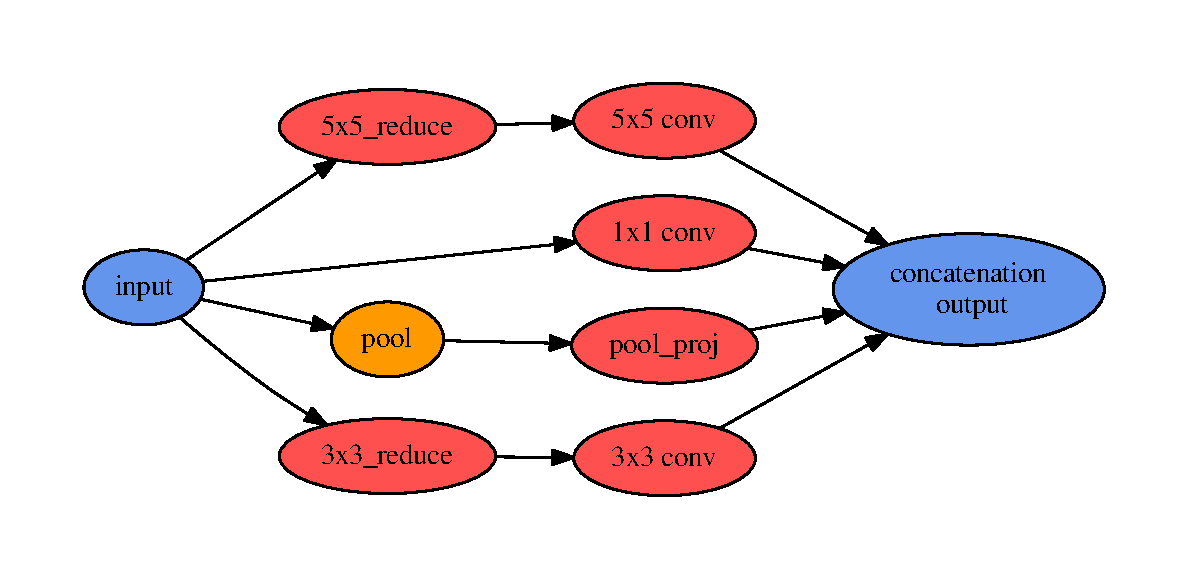
\includegraphics[scale=.45]{fig/inception.pdf}\\
  \caption{Inception Cell. $n\times n$ stands for size $n$ receptive field, $n\times n\_reduce$ stands for the $1\times 1$ convolutional layer before the $n\times n$ convolution layer and $pool\_proj$ is another $1\times 1$ convolutional layer after the MAX pooling layer. The output layer concatenates all its input layers.}\label{incept}
\end{figure}

\subsection{Food Datasets}
Besides ImageNet dataset, there are many popular benchmark datasets for image recognition such as Caltech dataset and CIFAR dataset, both of which contain hundreds of classes. However, in this paper, we try to focus on a more specific area, food classification. Compared to other recognition tasks, there are some properties of the food (dishes) which make the tasks become a real challenge:
\begin{itemize}
  \item Food doesn't have any distinctive spatial layout: for other tasks like scene recognition, we can always find some discriminative features such as buildings or trees, etc;
  \item Food class is a small sub-category among all the categories in daily life, so the inter-class variation is relatively small; on the other hand, the contour of a food varies depending on many aspects such as the point of the view or even its components.
\end{itemize}
So these properties make food classification catastrophic for some recognition algorithms. Therefore, the training these two architectures on the food recognition task can reveal some important aspects of themselves and help us better understand them. In this paper, we use two image datasets Food-256 \cite{kawano14c}\footnote{Dataset can be found http://foodcam.mobi/dataset.html} and Food-101 \cite{bossard14}\footnote{Dataset can be found http://www.vision.ee.ethz.ch/datasets\_extra/food-101}. It is worthy to mention that PFID dataset is also a big public image database for classification, but their images are collected in a laboratory condition which is considerably not applicable for real recognition task.

\textbf{Food-256 Dataset.}
This is a relatively small dataset containing 256 kinds of foods and 31644 images from various countries such as French, Italian, US, Chinese, Thai, Vietnamese, Japanese and Indonesia. The distribution among classes is not even and the biggest class (vegetable tempura) contains 731 images while the smallest one contains just 100 images. For this small dataset, we randomly split the data into training and testing set, using around 80\% (25361 images) and 20\% (6303 images) of the original data respectively and keep the class distribution in these two sets uniform. The collector of this dataset also provides boundary box for each image to separate different foods and our dataset is cropped according to these boundary boxes.

\textbf{Food-101 Dataset.}
This dataset contains 101-class real-world food (dish) images which were taken and labeled manually. The total number of images is 101,000 and there are exactly 1000 images for each class. Also, each class has been divided into training and testing set containing 750 images and 250 images respectively by its collector. The testing set is well cleaned manually while the training set is not well cleaned on purpose. This noisy training set is more similar to our real recognition situation and it is also a good way to see the effect of the noise on these two architectures.

Data argumentation is an efficient way to enrich the data. There are also some techniques that can applied to enlarge the dataset such as subsampling and mirroring. The original images are firstly resized to $256\times 256$ pixels. We crop the 4 corners and center for each image according to the input size of each model and flap the 5 cropped images to obtain 10 crops. For the testing set, the prediction of an image is the average prediction of the 10 crops.


\section{Experimental Discuss}\label{discuss}
Training a CNN with millions of parameters on a small dataset could easily lead to horrible overfitting. But the idea of supervised pre-training on some huge image datasets could preventing this problem in certain degree. Compared to other randomly initialized strategies with certain distribution, supervised pre-training is to initialize the weights according to the model trained from a specific task. Indeed, this initialization has certain bias as there is no single dataset including all the invariance for natural images \cite{agrawal2014analyzing}, but this bias can be reduced as the pre-trained image dataset increases and the fine-tuning should be benefit from this initialization.
\subsection{Pre-training and Fine-tuning}
We conduct several experiments on both architectures and use different training initialization strategies for both Food-256 and Food-101 datasets. The scratch models are initialized with Gaussian distribution for AlexNet and Xavier algorithm for GoogLeNet%, which automatically determines the scale of initialization based on the number of input and output neurons
 \cite{glorot2010understanding}. These two initializations are used for training the original models for the ImageNet task. The ft-last and fine-tuned models are initialized with the weights pre-trained from ImageNet dataset. For the ft-last model, we just re-train the softmax layers while the whole network is fine-tuned for the fine-tune model.
\begin{table}[htbp]
  \centering
  \caption{Top-5 Accuracy in percent on fine-tuned, ft-last and scratch model for two architectures}
    \begin{tabular}{r|cc|cc}
    \toprule
          & \multicolumn{2}{c|}{AlexNet} & \multicolumn{2}{c}{GoogLeNet} \\    \midrule
     & Food-101   & Food-256   & Food-101   & Food-256 \\
    Fine-tune & \textbf{88.12} & \textbf{85.59} & \textbf{93.51} & \textbf{90.66} \\
    Ft-last &76.49	&79.26&	82.84	&83.77\\
    Scratch & 78.18 & 75.35 & 90.45 & 81.20 \\
    \bottomrule
    \end{tabular}%
  \label{tab:ft}%
\end{table}%

% Table generated by Excel2LaTeX from sheet 'Sheet1'
\begin{table*}[htbp]
  \centering
  \caption{Top-1 accuracy compared to other methods on Food-101 dataset in percent}
    \begin{tabular}{c|C{3cm}C{3cm}cc}
    \toprule
          & RFDC\cite{bossard14} & MLDS($\approx$\cite{singh2012unsupervised}) & GoogLeNet & AlexNet \\
    \midrule
    Top1 accuracy & 50.76 & 42.63& \textbf{78.11 }& 66.40 \\
    \bottomrule
    \end{tabular}%
    \label{tab:101}
\end{table*}%
% Table generated by Excel2LaTeX from sheet 'Sheet1'
\begin{table}[htbp]
  \centering
  \caption{Accuracy compared to other method on Food-256 dataset in percent}
    \begin{tabular}{cC{3cm}cc}
    \toprule
     & fv+linear \cite{Kawano:2014} & GoogLeNet & AlexNet \\
     
    \midrule
    top1  & 50.1& \textbf{70.1} & 63.8 \\
    top5  & 74.4  & \textbf{90.6} & 85.6\\
    \bottomrule
    \end{tabular}%
  \label{tab:256}%
\end{table}%


\begin{figure*}[htbp]
  \centering
  % Requires \usepackage{graphicx}
  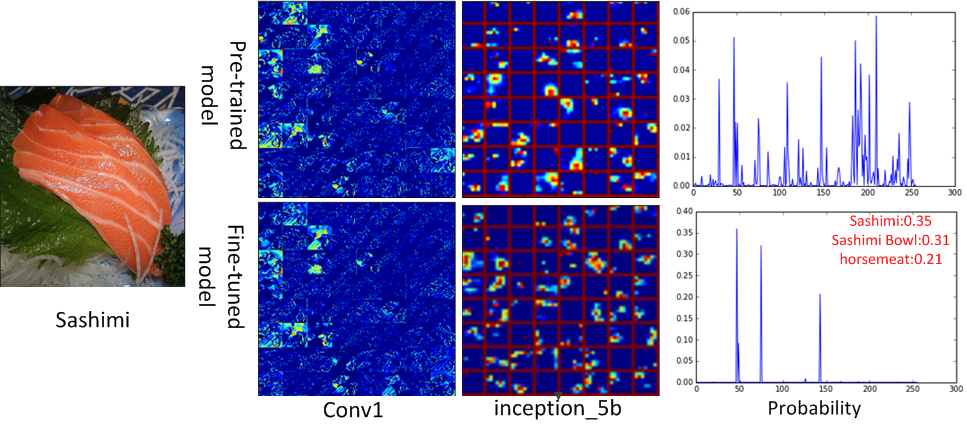
\includegraphics[scale=0.5]{fig/sashimi.png}\\
  \caption{Visualization of some feature maps of different GoogLeNet models in different layers for the same input image. 64 feature maps of each layer are shown. Conv1 is the first convolutional layer and Inception\_5b is the last convolutional layer. }
   \label{fig:sashimi}
\end{figure*}
From Table \ref{tab:ft} we can see that fine-tuning the whole network can improve the performance of the CNN for our task. Compared to other traditional computer vision methods (see Table \ref{tab:101} and \ref{tab:256}), GoogLeNet outperforms the other methods with large margins and we provide the state-of-the-art performance of these two food image datasets.

In Figure \ref{fig:sashimi} we visualize the feature maps of the pre-trained GoogLeNet model and fined-tuned GoogLeNet model with the same input image for some layers. We can see that the feature maps of the lower layer are similar as the lower level features are similar for most recognition tasks.
Then we can see that the feature maps in the high-level are different which leads to totally different recognition results.
Since only the last layer (auxiliary classifier) of the ft-last model is optimized, we can infer that the higher level features are more important which is consistent with our intuition. Also from Table \ref{tab:ft}, it is interesting to see that for the Food-101 task, the accuracy of  the scratch models outperforms the pre-trained models. Since Food-101 is a relatively large dataset with 750 images per class while Food-256 dataset is an imbalanced small one, this indicates that it is difficult to obtain a good deep CNN model while the data is insufficient.

From Table \ref{tab:ft} we can see that GoogLeNet always performances better than AlexNet on both datasets. This implies that the higher level features of GoogLeNet are more discriminative compared to AlexNet and this is due to the special architecture of its basic unit, Inception. Table \ref{tab:cosg} and \ref{tab:cosa} show the weights' cosine similarity of each layer between the fine-tuned models and their pre-trained models. From the results we can see that the weights in the low layer are more similar which implies that these two architectures can learn the hierarchical features. As the low level features are similar for most of the tasks, the difference of the objects is determined by high-level ones which are the combination of these low level features. Also from Table \ref{tab:cosa}, we can observe that, the weights of the pre-trained and fine-tuned models are extremely similar in AlexNet . This can be caused by two reasons:
\begin{itemize}
  \item Size of receptive filed. Since ReLUs are used in both architectures, vanishing gradients do not exist. Rectified activation function is mathematically given by:
      \begin{equation}\label{relu}
        h = \max ({w^T}x,0) = \left\{ {\begin{array}{*{20}{c}}
{{w^T}x}&{{w^T}x > 0}\\
0&{else}
\end{array}} \right.
      \end{equation}

    The ReLU is inactivated when its input is below 0 and its partial derivative is 0 as well. Sparsity can boost the performance of the linear classifier on top, but on the other hand, sparse representations make the network more difficult to train as well as fine-tuning. The derivative of the filter is $\frac{{\partial J}}{{\partial w}} = \frac{{\partial J}}{{\partial y}}\frac{{\partial y}}{{\partial w}} = \frac{{\partial J}}{{\partial y}}*x$ where $\frac{{\partial J}}{{\partial y}}$ denotes the partial derivative of the activation function, $y=w^Tx$ and $x$ denotes the inputs of the layer. The sparseness of the input could lead to sparse filter derivative for back propagation. Therefore, the filters of the fine-tuned AlexNet is extremely similar. Compared to large receptive field used in AlexNet, the inception in GoogLeNet employs 2 additional $n\times n\_reduced$ convolutional layers before the $3\times 3$ and $5\times 5$ convolutional layers (see Figure \ref{incept}). Even though the original purpose of these two $1\times 1$ convolutional layer is for computational efficiency, these 2 convolutional layers tend to squeeze their sparse inputs and generate a dense outputs for the following layer. This makes the filters in the following layer more easily to be trained for transfer learning and generate efficient sparse representations.
  \item The pooling strategy. In AlexNet, max pooling is applied to all the pooling layers between several convolution layers and in back propagation, the max pooling layer always passes the error to the place where it came from. Since it only came from one place of the receptive field, the back propagation error is sparse and keeps the most filters' weights unchanged. In GoogLeNet, even though, there is a max pooling layer within every inception, there are other 3 back propagation errors, from $5\times 5\_reduce$ and $3\times 3\_reduce$ that can affect the weights of the previous inception.
\end{itemize}

\begin{table*}[htbp]
  \centering
  \caption{Cosine similarity of the inceptions between fine-tuned models and pre-trained model for GoogLeNet}
    \begin{tabular}{r|cccccc}
    \toprule
    \multicolumn{7}{c}{food256} \\
    \midrule
          & \multicolumn{1}{l}{1x1} & \multicolumn{1}{l}{3x3\_reduce} & \multicolumn{1}{l}{3x3} & \multicolumn{1}{l}{5x5\_reduce} & \multicolumn{1}{l}{5x5} & \multicolumn{1}{l}{pool\_proj } \\
    inception\_3a & 0.72  & 0.72  & 0.64  & 0.67  & 0.73  & 0.69 \\
    inception\_3b & 0.59  & 0.64  & 0.53  & 0.70  & 0.60  & 0.56 \\
    inception\_4a & 0.46  & 0.53  & 0.54  & 0.50  & 0.67  & 0.38 \\
    inception\_4b & 0.55  & 0.58  & 0.63  & 0.52  & 0.69  & 0.41 \\
    inception\_4c & 0.63  & 0.64  & 0.63  & 0.57  & 0.68  & 0.52 \\
    inception\_4d & 0.60  & 0.62  & 0.60  & 0.58  & 0.68  & 0.50 \\
    inception\_4e & 0.60  & 0.61  & 0.67  & 0.61  & 0.68  & 0.50 \\
    inception\_5a & 0.51  & 0.53  & 0.58  & 0.48  & 0.60  & 0.39 \\
    inception\_5b & 0.40  & 0.44  & 0.50  & 0.41  & 0.59  & 0.40 \\  \toprule
    \multicolumn{7}{c}{food101} \\ \midrule
          & \multicolumn{1}{l}{1x1 } & \multicolumn{1}{l}{3x3\_reduce} & \multicolumn{1}{l}{3x3} & \multicolumn{1}{l}{5x5\_reduce} & \multicolumn{1}{l}{5x5} & \multicolumn{1}{l}{pool\_proj } \\
    inception\_3a & 0.71  & 0.72  & 0.63  & 0.67  & 0.73  & 0.68 \\
    inception\_3b & 0.56  & 0.63  & 0.50  & 0.71  & 0.60  & 0.53 \\
    inception\_4a & 0.43  & 0.50  & 0.50  & 0.47  & 0.62  & 0.36 \\
    inception\_4b & 0.48  & 0.52  & 0.57  & 0.50  & 0.67  & 0.35 \\
    inception\_4c & 0.57  & 0.61  & 0.59  & 0.53  & 0.63  & 0.47 \\
    inception\_4d & 0.54  & 0.58  & 0.53  & 0.54  & 0.64  & 0.44 \\
    inception\_4e & 0.53  & 0.54  & 0.61  & 0.55  & 0.62  & 0.42 \\
    inception\_5a & 0.43  & 0.47  & 0.53  & 0.45  & 0.57  & 0.34 \\
    inception\_5b & 0.36  & 0.39  & 0.46  & 0.38  & 0.52  & 0.37 \\
    \bottomrule
    \end{tabular}%
  \label{tab:cosg}%
\end{table*}%


\begin{table*}[htbp]
  \centering
  \caption{Cosine similarity of the layers between fine-tuned models and pre-trained model for AlexNet}
    \begin{tabular}{r|ccccccc}
    \toprule
          & conv1 & conv2 & conv3 & conv4 & conv5 & fc6   & fc7 \\
    \midrule
    food256 & 0.997 & 0.987 & 0.976 & 0.976 & 0.978 & 0.936 & 0.923 \\
    food101 & 0.996 & 0.984 & 0.963 & 0.960 & 0.963 & 0.925 & 0.933 \\
    \bottomrule
    \end{tabular}%
  \label{tab:cosa}%
\end{table*}%

% Table generated by Excel2LaTeX from sheet 'google'
\begin{table*}[htbp]
  \centering
  \caption{Sparsity of the output for each unit in GoogLeNet inception for training data from Food101 in percent}
    \begin{tabular}{r|cccccc}
    \toprule
          & 1x1  & 3x3\_reduce & 3x3  & 5x5\_reduce & 5x5  & pool\_proj  \\
    \midrule
    inception\_3a & $69.3\pm 1.3$  & $69.6 \pm 1.1$  & $80.0\pm  1.0$& $64.1\pm  2.2$& $75.8\pm  1.6$& $76.2\pm 5.4$\\
    inception\_3b & $92.8 \pm 0.9$&$ 76.5 \pm 0.9$& $94.7\pm 0.9 $&$ 71.6 \pm 2.3 $&$ 94.4\pm 0.5 $&$ 94.7 \pm 1.6$\\
    inception\_4a & $90.9 \pm 0.9$& $70.0\pm 1.2 $& $93.8\pm 1.1 $& $63.3\pm 4.0 $& $91.9\pm 1.8 $& $95.1\pm 2.0$\\
    inception\_4b & $71.9 \pm 1.6$& $67.5\pm 1.2$ & $75.4\pm  1.0$& $58.5 \pm 2.6$& $78.9\pm  1.6$& $85.6\pm 3.6$\\
    inception\_4c & $75.1 \pm 2.4$& $72.6 \pm 1.3$& $81.0\pm 2.0$ & $66.3\pm 6.1 $& $79.7 \pm 3.6$& $88.1\pm 3.3$\\
    inception\_4d & $87.3 \pm 2.7$& $78.0 \pm 2.2$& $88.0\pm 1.6$& $67.9\pm 3.1 $& $88.9\pm 2.8 $& $93.0\pm 2.2$\\
    inception\_4e & $91.8\pm  1.1$& $62.3\pm 2.2 $& $91.0\pm 2.5 $& $49.5 \pm 3.7$& $94.0 \pm 1.0$& $92.3\pm 1.5$\\
    inception\_5a & $78.7 \pm 1.6$& $66.5\pm  1.7$& $82.3\pm 2.6 $& $59.9\pm 3.2 $& $86.4\pm 2.3 $& $87.1\pm 2.6$\\
    inception\_5b & $88.2\pm 2.3 $& $86.8 \pm 1.6$&$ 83.3\pm 4.4$ & $84.0\pm 3.1 $& $81.4\pm 5.3$  & $94.7\pm 1.5$\\
    \bottomrule
    \end{tabular}%
  \label{tab:addlabel}%
\end{table*}%

The unique structure of the Inception guarantees that the sparse outputs from previous layer can be squeezed with the $1\times 1$ convolutional layers and feed to convolutional layers with bigger receptive field to generate sparser representation. The squeeze action promises the back propagation error can be transferred more efficiently and makes the whole network more flexible to fit different recogntion tasks.

\subsection{Learning across the datasets}
From the previous experiments we can see that pre-training on the ImageNet dataset can improve the performance of the deep convolutional neural network on our specific area. In this part, we will discuss the generalization ability within the food recognition problem.  Zhou et al. trained AlexNet for Scene Recognition across two datasets with identical categories \cite{NIPS2014_Zhou}. But for more complex situation, such as two similar datasets with a little overlapped categories, we are very interested in exploring whether deep CNN can still successfully handle. Therefore, we conduct the following experiment to stimulate a more challenging real world problem: transferring the knowledge from the fine-tuned Food-101 model to a target set, Food-256 dataset. To make the experiment more practical, we limit the number of samples per category from Food-256 for training, because if we want to build a our own model using deep CNN for a specific task, the resource is always limited and it is exhausted to collect hundreds of labeled images for each category.

The Food-101 and Food-256 datasets share about 46 categories of food even though the images in the same category may vary across these two datasets. The types of food in Food-101 are mainly western style while most types of food in Food-256 are typical Asian foods. We compare the top-5 accuracy trained from different size of subset for Food-256 on different pre-trained model and the results are shown in Table \ref{tab:cross}.
%The ImageNet columns denote  the pre-trained model trained only on ImageNet images and the Food101\_ft columns denote the pre-trained model trained on ImageNet images and then fine-tuned on Food-101.
The ImageNet columns denote using the model pre-trained from ImageNet dataset as the pre-trained model and Food101\_ft columns denote using the fine-tuned Food-101 model (the same one in Table \ref{tab:ft}) as the pre-trained model.

From the result of Table \ref{tab:cross} we can see that, with this further transfer learning, both CNNs can achieve around 95\% of the accuracy trained on full dataset while just utilizing about half of them (50 per class, 12800 of 25361 images). This indicates that when there is not enough labeled data, with its strong generalization ability, deep CNN trained from general task can still achieve satisfying result and perform even better when an additional relevant dataset is involved. This encouraging result may attract more people to use deep CNN for their specific task and continue to explore the potential of the existing architecture as well as designing new ones.

\begin{table*}[htbp]
  \centering
  \caption{Top5 Accuracy for transferring from Food101 to subset of Food256 in percent}
    \begin{tabular}{c|cc|cc}
    \toprule
          & \multicolumn{2}{c|}{AlexNet} & \multicolumn{2}{c}{GoogLeNet} \\
    \midrule
    instances per class & ImageNet  & Food101\_ft    &  ImageNet  & Food101\_ft \\ \midrule
    20    & 68.80  & {75.12} & 74.54 & {77.77} \\
    30    & 73.15 & {77.02} & 79.21 & {81.06} \\
    40    & 76.04 & {80.23} & 81.76 & {83.52} \\
    50    & 78.90  & {81.66} & 84.22 & {85.84} \\
    all    & 85.59 &  {87.21} & {90.66 }&   {90.65}     \\
    \bottomrule
    \end{tabular}%
  \label{tab:cross}%
\end{table*}%



\section{Conclusion}
In this paper, we compare two different deep convolutional neural network architectures and their transferring ability on food datasets. Both architectures have shown their potential on generalization ability and we provide the-state-of-the-art on Food-101 dataset and competitive baseline on Food-256 dataset using fine-tuned GoogLeNet. GoogLeNet shows its strong ability on transferring the knowledge between different tasks with the help of the specially designed unit, Inception. 
%Intensively used $1\times 1$ convolutional layer in Inception reduces both computational cost and training complexity which leads to the final success of the whole architecture.  
We find that not only does the intensively used $1\times 1$ convolutional layer in Inception reduce the computational cost, but it also helps to train the filters in the following layer. The filters after the $1\times 1$ convolutional layer can be trained more efficiently while the $1\times 1$ convolutional layer provides squeezed input and this feature helps GoogLeNet learn more complex high-level features.
Moreover, in a more practical situation such as transfer learning within a specific area with a few labeled instances for the target set, both of these two architectures show some encouraging result in transferring knowledge across the dataset, reaching around 95\% of the accuracy trained on full dataset with just half data.



% Acknowledgements should only appear in the accepted version.
\section*{Acknowledgments}




% In the unusual situation where you want a paper to appear in the
% references without citing it in the main text, use \nocite
\nocite{langley00}

\bibliography{research}
\bibliographystyle{icml2015}

\end{document}


% This document was modified from the file originally made available by
% Pat Langley and Andrea Danyluk for ICML-2K. This version was
% created by Lise Getoor and Tobias Scheffer, it was slightly modified
% from the 2010 version by Thorsten Joachims & Johannes Fuernkranz,
% slightly modified from the 2009 version by Kiri Wagstaff and
% Sam Roweis's 2008 version, which is slightly modified from
% Prasad Tadepalli's 2007 version which is a lightly
% changed version of the previous year's version by Andrew Moore,
% which was in turn edited from those of Kristian Kersting and
% Codrina Lauth. Alex Smola contributed to the algorithmic style files.
